        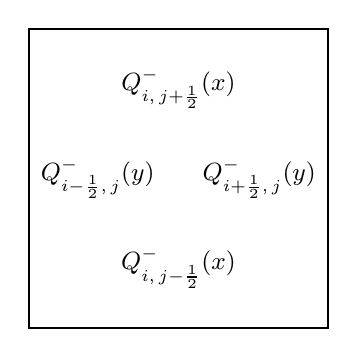
\begin{tikzpicture}[font=\small]
            \def\L{3.8}
    
            % Cell boundary
            \draw[line width=0.9pt] (0,0) rectangle (\L,\L);
    
            % % Corner coordinate labels (outside the cell)
            % \node[anchor=south east] at (0,\L)
            %     {\footnotesize$(x_{i-\frac{1}{2}},\,y_{j+\frac{1}{2}})$};
            % \node[anchor=south west] at (\L,\L)
            %     {\footnotesize$(x_{i+\frac{1}{2}},\,y_{j+\frac{1}{2}})$};
            % \node[anchor=north east] at (0,0)
            %     {\footnotesize$(x_{i-\frac{1}{2}},\,y_{j-\frac{1}{2}})$};
            % \node[anchor=north west] at (\L,0)
            %     {\footnotesize$(x_{i+\frac{1}{2}},\,y_{j-\frac{1}{2}})$};
    
            % Trace labels inside the cell
            \node at (0.50*\L, 0.80*\L)
                {$\bm{Q}^-_{i,\,j+\frac{1}{2}}(x)$};
            \node at (0.50*\L, 0.20*\L)
                {$\bm{Q}^-_{i,\,j-\frac{1}{2}}(x)$};
            \node at (0.23*\L, 0.50*\L)
                {$\bm{Q}^-_{i-\frac{1}{2},\,j}(y)$};
            \node at (0.77*\L, 0.50*\L)
                {$\bm{Q}^-_{i+\frac{1}{2},\,j}(y)$};
        \end{tikzpicture}